\setcounter{section}{17}
\section{Операции над множествами (масками): объединение, пересечение, разность. Реализация в программе. Проверка, что одна маска является подмножеством другой. Проверка, что число является
степенью двойки.}
Идея ДП по маскам: пусть n какое-то небольшое число ($\leq$ 30-60), тогда мы можем эффективно закодировать все подмножества множества $\{0,...,n-1\}$. Для этого рассматриваем маску. Она будет состоять из n символов, каждый из которых - единица или ноль. Единица на i-м месте в маске означает, что мы берем число i в подмножество, 0 - не берем в подмножество
\subsection*{Операции над масками}
Пусть даны два множества А и В с соответсвующими им масками $mask_A$ и $mask_B$ ($\oplus$ = xor)
\begin{itemize}
    \item []\textbf{Объединение}\\  $A \cup B = mask_A \ | \ mask_B$
     \item []\textbf{Пересечение} \\ $A \cap B = mask_A \ \& \ mask_B$
     \item []\textbf{Разность} $A \backslash B = (mask_A \ | \ mask_B) \ \oplus \ mask_B = mask_A \&(\sim mask_B)$.  \begin{center}
         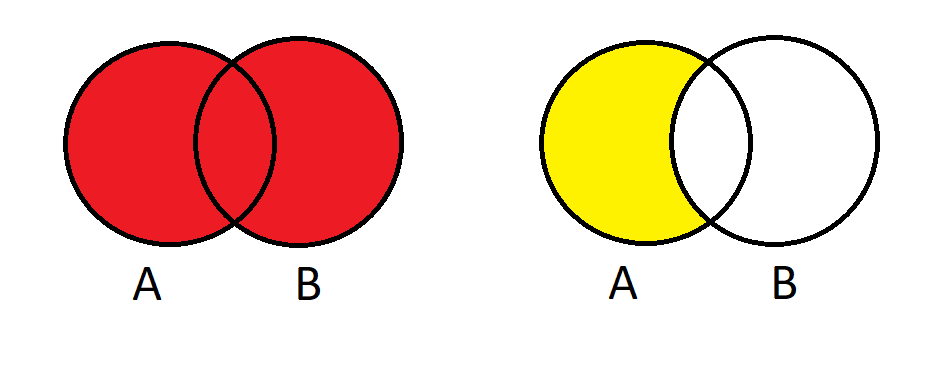
\includegraphics[width = 17cm]{images/18-24_alg1.PNG}
          $mask_A \ | \ mask_B$ \ \ \ \ \ \ \ \  \ \ \ \ \ \ \ \ \ \ \ \ \ \ \ \ \ \ \ \ \ \ $(mask_A \ | \ mask_B) \ \oplus \ mask_B$ \ \ 
     \end{center} 
\end{itemize}

\subsection*{Проверка, что одна маска является подмножеством другой}
Пусть даны две маски A и B. Утверждается, что $B \subset A \Longleftrightarrow (A \& B) = B \\ \blacktriangle \\ \rightarrow$ Пусть $B \subset A$, тогда если в маске B на месте i стоит единица, то и в маске А на месте i стоит единица, а значит, их побитовое "и" даст в точности В. \\$\leftarrow$ Если $(A \& B) = B$, то в маске A единицы стоят как минимум на тех местах, что и в маске В, иначе их побитовое "и" не дало бы единицу на том же месте, что и в маске В. Это значит, что $B \subset A \ \blacksquare $ 

\subsection*{Проверка, что число является степенью двойки.}
Утверждается, что число a является степенью двойки $\Longleftrightarrow a \& (a-1) = 0 \\ \blacktriangle \\ \rightarrow$ Рассмотрим двоичную запись числа а. Если а = $2^n$, то a = $1\underbrace{0...0}_{n} \Longrightarrow \ a - 1 = \underbrace{1...1}_{n-1} \Longrightarrow a \&(a-1) = 0 \\ \leftarrow$ Пусть $a \neq 1\underbrace{0...0}_{n}$, тогда $a = \underset{n}{1} ...1\underbrace{...}_{i-1}$, т.е. существует единица на i-м месте в записи числа а, тогда $a - 1 = \underset{n}{1} \underbrace{...}_{n-1}$, т.е. старший бит не обнуляется, а значит, побитовое "и" не может равняться нулю. Противоречие. $\blacksquare$
\setcounter{section}{18}
\section{Задача о самом дешёвом гамильтоновом пути: решение за O($2^n n^2$)}

Запишем важную и полезную функцию, которая позволяет извлекать i-й элемент маски:
\begin{lstlisting}
bool bit(long long mask, int pos) {
	return (mask >> pos) & 1;
}
\end{lstlisting}
\textbf{Формулировка задачи} \\ Дан полный, неориентированный, взвешанный граф.
\\
\textit{Гамильтонов путь в графе} - это путь, который начинается в какой-то вершине графа, проходит по всем вершинам и посещает все вершины графа ровно по одному разу
\\
Среди всех таких путей нас интересует путь минимальной стоимости
\\
\\
\\
Пусть у нас есть какой-то путь, проходящий по каким-то вершинам графа ровно один раз и заканчивающийся в вершинке v. Тогда для того, чтобы продолжить этот путь, нам необходимо знать, в какой вершинке мы находимся и маску посещенный вершин. Отсюда возникает dp:
\\
\\
1. dp[v][mask] - это стоимость минимального пути, который где-то начинается, посещает все вершины маски ровно по одному разу и заканчивается в v\\
2. База: Пути длины 0. Когда мы стоим в какой-то вершинке и еще никуда не пошли. \\ dp[v][$2^v$] = 0, все остальные значения положим $+\infty$ \\
3. Переход: перебираем все ребра, исходящие из v, которые ведут в вершины, еще не посещенные (в маске на месте соответствующей вершины будет стоять 0), и смотрим, куда можем пойти. 
\\
\\
 (1<<u)|mask - взять побитовое "или" числа $2^u$ и mask. Нетрудно заметить, что такая процедура просто ставит единичку на u-й бит маски
\begin{lstlisting}
for (int mask = 0; mask < 2^n; ++mask){
    for(int v = 0; v < n; ++v){
        for(int u = 0; u < n; ++u){
            if(bit(mask,u)) continue;
            int newmask = (1<<u)|mask;
            dp[u][newmask] = max(dp[u][newmask], dp[v][mask] + cost[v][u]);
        }
    }
}
\end{lstlisting}
4. Ответ: Минимальное $dp[u][2^n - 1]$. То есть нас интересуют все пути, которые посещают все вершины, выбираем из них тот, что имеет минимальную стоимость
\\

\textbf{Асимптотика}
\\
За счет циклов $O(2^n n^2)$

\setcounter{section}{19}
\section{Задача о максимальной клике: решения за $O(2^nn^2)$, $O(2^nn)$, $O(2^n)$}
\textbf{Формулировка задачи} \\ Дан неориентированный, взвешанный граф.
\\
\textit{Кликой} в неориентированном графе называется подмножество вершин, каждые две из которых соединены ребром графа.
\\ 
\\ Хотим найти максимальную по мощности клику в данном графе

\subsection*{$O(2^nn^2)$}
Перебираем все подмножества n и за $n^2$ перебором проверяем, что это клика

\subsection*{$O(2^nn)$}
1. Положим $dp[mask] = \begin{cases}
   true &   mask - klika\\
   false &   else
 \end{cases}$

2. Будем делать дп назад

3. $dp[mask]$ - клика $\Longleftrightarrow$ для любой вершины v из этой маски выполнено:
\begin{itemize}
    \item [1] $dp[mask \oplus 2^v] = true$. $mask \oplus 2^v$ - на v-ое место маски ставит false. Здесь мы проверяем, что маска без этой вершинки v - клика 
    \item[2] v соединена со всеми вершинами маски
\end{itemize}
4. База: dp[0] =  true\\
5. Ответ: максимальная по мощности маска, для которой dp[mask] = true\\
\textbf{Асимптотика}\\
Перебор всех масок: $2^n$. Для каждой маски необходимо за линейное время определить какую-нибудь вершинку, которая входит в эту маску (просто пройтись по n битам и найти тот, для которого bit(mask, i) = true). Далее идем по маске и за линейное время определяем, связана ли вершинка, которую мы выбрали, со всеми остальными. Итого получаем  O($2^n n$)

\subsection*{$O(2^n)$}
Новый алгоритм - это оптимизация предыдущего. 
\begin{itemize}
    \item [1] Для каждой вершинки u посчитаем маску ее соседей. Пусть  neigh[u] - маска соседей u. Сделаем это на этапе ввода графа.
    \item[2]  Теперь бит v выбираем не произвольным образом. Это будем старший включенный бит маски. Почему старший? Его будет удобно насчитывать, что мы поймем дальше
    \end{itemize}
 Тогда проверка пункта 3.2(см. предыдущий алгоритм) будет проверяться за О(1): \\ dp[$mask \oplus 2^v$] $\subset neigh[v]$. Из 18 билета мы знаем, что $a \subset b \Longleftrightarrow (a \ \& \ b) = a$. Значит, проверка:\\$(dp[mask \oplus 2^v] \  \&  \ neigh[v]) = dp[mask \oplus 2^v]$
 \\
 \\
 Теперь поймем, как хранить старший бит
 \begin{lstlisting}
 int oldest_bit = -1;
 for(int mask = 1; mask < 2^n; ++mask){
    if(mask & (mask - 1) == 0) ++oldest_bit;
    ...
 }
 \end{lstlisting}
 Сначала отметим старший бит равным -1. Очевидно, что старший бит маски будет меняться только в том случае, если мы переходим через степень двойки ($mask \  \& (mask - 1) == 0$ - проверка на то, что mask - степень двойки, см. 18 билет)
 \\
 \\
 \textbf{Асимптотика}\\
 Таким образом, мы научились делать переход за O(1). Значит, итоговая асимптотика O($2^n$) 

 \setcounter{section}{20}
\section{Подсчёт всех значений \texorpdfstring{$b(mask) = \max_{s \subset mask} a(s)$}{b(mask)} для данного набора значений $a(0), a(1), ..., a(2^n-1)$ за $O(2^nn)$}
 Мы хотим для каждой из масок 0...$2^n - 1$ посчитать максимальное по мощности подмножество маски, являющееся кликой
 Пусть a(V) = 
 \begin{itemize}
     \item [] 0, если V - не клика
     \item[]|V|, если V - клика
 \end{itemize}
 Тоогда мы хотим найти   b(mask) = $\underset{V \subset mask}{max} \ a(V)$. Будем делать это с помощью дп\\
 1. dp[k][mask] = $\underset{V \subset mask}{max} \ a(V)$, где V - такое, что первые k битов V и mask совпадают \\
 2. База dp[n][mask] = a(mask)\\
 3. Переход. Будем ходить по подмаскам. Пусть нам известно dp[i+1][mask]. Научимся преходить к dp[i][mask]. Зафиксируем старшие i битиков, тогла номер у следующего, если считать от начала маски, n-i-1 
 \begin{center}
     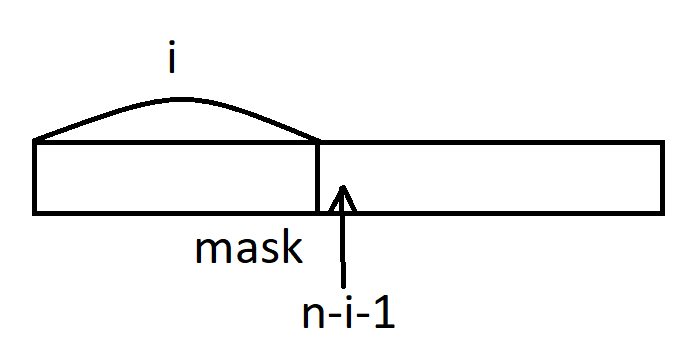
\includegraphics[width=17cm]{images/18-24_alg4.PNG}
 \end{center}
 \begin{itemize}
     \item [1]  Если !bit(mask, n - i -1), то при переходе к подмаске мы не убрали ни одного элемента (т.к. при переходе к подмаске 0 не может стать единицей, значит, остается только 0), а значит, максимальная мощность подмножества, являющегося кликой, не изменилась, dp[i][mask] = dp[i+1][mask]
     \item [2]  Если bit(mask, n -i-1), то у нас есть выбор, при переходе к подмаске оставить единицу на этом месте или превратить ее в ноль. Так как мы ищем максимальную мощность, то dp[i][mask] = max(dp[i+1][mask], dp[i][$mask \oplus 2^{n - i- 1}$]
 \end{itemize}
 4. Ответ: b(mask) = dp[0][mask]\\
 \textbf{Асимптотика}\\ 
 1. Базу можно насчитать за O($2^n$)\\
 2. Перебираем все i = n-1...0, перебираем все маски, делаем переход за O(1)
 \\
 Итог: O($2^n n$)
 
\setcounter{section}{21}
\section{Задача о максимальной клике: решение за O($2^{\frac{n}{2}} n$).}
 Здесь будет использоваться идея meet-in-the-middle. Она заключается в том, что мы делим n пополам и получаем две маски длины $\frac{n}{2}$
 \begin{center}
     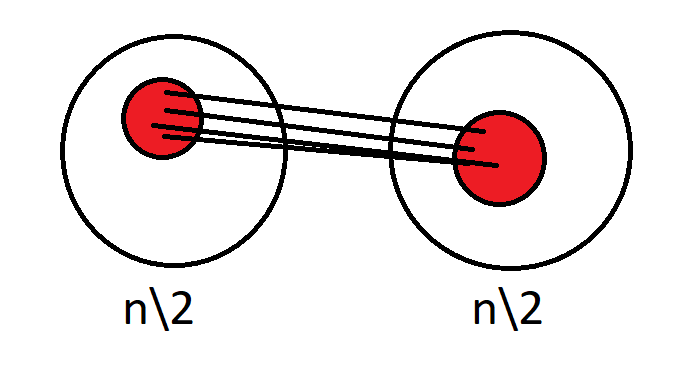
\includegraphics[width=17cm]{images/18-24_alg2.PNG}
 \end{center}
  Очевидно, что если маска является кликой, то, если мы распилим ее пополам, новые маски останутся тоже кликами.\\  Если мы нашли какую-то клику в одном из множеств, то, если мы дополним ее нулями, получится клика во множестве масок длины n.
  \\
  \\ Отсюда получаем, что все маски длины n можно разделить на 3 группы
  \begin{itemize}
      \item [1] Правая часть - нули, левая - клика в левом множестве
      \item [2] Левая часть - нули, правая - клика в правом множестве
      \item[3] u (левая часть маски длины n) - клика в левом множестве, v (правая часть маски длины n) - клика в правом множестве
  \end{itemize}
\textbf{Алгоритм} \\
Рассмотрим маску вершин левой доли mask. И запишем маску mask\_right вершин правой доли, которые соединены со всеми вершинами из mask. (То есть перебираем все вершины правой доли, и если какая-то вершина соединена со всеми из mask, добавляем ее в маску mask\_right)
\\
\\ 
Пусть dp1[mask] = mask\_right, neigh'[v] - маска соседей v в правой доле (вершина v из левой доли), посчитать все neigh'[i] можно за квадрат простым перебором\\
1. dp1[0] - вся правая доля\\
2. Хотим добавить в маску вершинку v. dp1[mask|$2^v$] = (dp1[mask]\& neigh'[v])
\begin{center}
    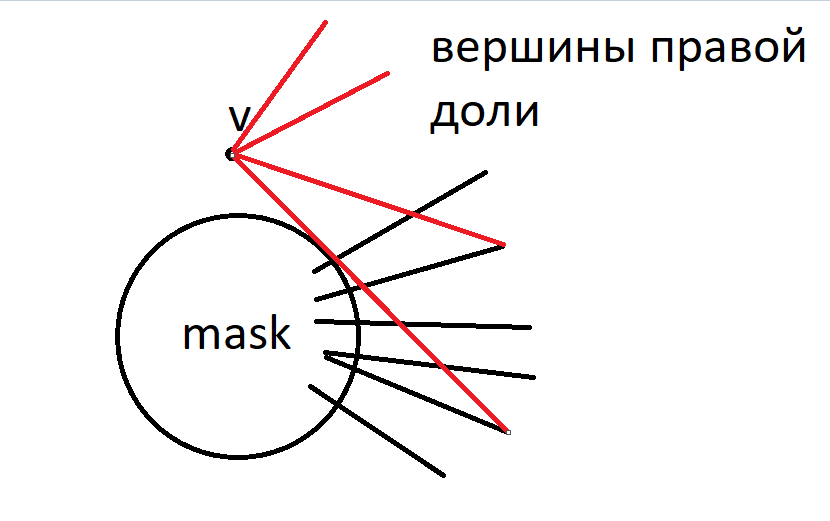
\includegraphics[width=17cm]{images/18-24_alg3.PNG}
\end{center}
В маску dp1[mask|$2^v$] входит персечение соседей v и соседей всех вершин mask. По определению пересечение всех соседей mask - это dp1[mask]
\\
\\ Зафиксируем множество U, являющееся кликой в левой доле. Тогда дополнение V множества U до клики во всем множестве - это некоторое подмножество dp1[U]. Поскольку U - клика, и из U проведены все ребра в вершины правой доли, то V - это максимальное подмножество dp1[U], которое является кликой (так как все остальные вершины соединены между собой, осталось найти множество вершин из dp1[U], которые соединены между собой). 
\\
\\ Для любой маски mask правой доли найдем максимальное по мощности множество $V \subset mask$, являющееся кликой. Будем это делать, используя алгоритм из билета 21, за $2^{\frac{n}{2}} n$\\
\textbf{Асимптотика}\\
1. Насчитать dp1[mask] - перебор всех масок за $2^{\frac{n}{2}}$, для каждой маски проходимся по всем вершинам левой доли от 0...$\frac{n}{2}$, проверяем, входит ли вершина в mask O(1), если не входит, то делаем переход по формуле за O(1). Тогда этот шаг за O($2^{\frac{n}{2}}n$)\\  
2. Насчитать для каждой маски mask правой доли максимальную клику a[mask], являющуюся подмаской за O($2^{\frac{n}{2}}n$)\\
3. Перебираем все маски mask левого множества, являющиеся кликами(можно воспользоваться алгоритмом за $2^n$ или $2^n n$, там будет насчитано нужное dp), для каждого dp1[mask] максимальная клика в правом множестве - a[dp1[mask]], тогда искомое множество - объединение mask и a[dp1[mask]]. Мощность объединения можно посчитать за O(n), насчитывая количество единиц в двоичной записи масок. Третий шаг за O($2^{\frac{n}{2}}n$)
\\
Итоговая асимптотика: O($2^{\frac{n}{2}}n$)

\setcounter{section}{22}

\section{Симпатичные узоры: количество раскрасок таблицы n × m в два цвета без одноцветных квадратиков 2 × 2. Прямой профиль: решения за O($4^n(n+m)$) и O($8^nlog m$)}

\subsection*{O($4^n(n+m)$)}

\textbf{Формулировка}\\ 
Дана таблица nxm и два цвета
\begin{itemize}
    \item [1] - черный
    \item [2] - белый
\end{itemize}
Мы не хотим, чтобы в таблице были квадратики 2х2, расскрашенные в один цвет
\\ Сколько есть таких раскрасок? \\ \\
Предположим, мы уже раскрасили j столбцов. Что нам нужно знать для продолжения раскраски? Очевидно, нам нужно знать только цвета последнего столбца. Отсюда возникает динамика:
\\
\\1. dp[j][mask] - сколько есть раскрасок j  столбцов так, чтобы последний из них был в точности покрашен в mask\\
2. Переход: перебираем все маски, соответствующие расскраске следующего слолбца и смотрим, не нарушается ли симпатичность узора 
\\
\\
Предподсчитаем корректность перехода между масками. Для этого перебираем все комбинации масок и проверяем, сравнивая их за O(n), корректен ли переход. асимптотика предподсчета O($4^n n$)
\\
3.База: dp[1][mask] = 1\\
4.Ответ: сумма по всем i dp[m][i]
\\
\begin{lstlisting}
for (int j = 1; j <= m - 1; ++j) {
	for (long long mask = 0; mask < 2^n - 1; ++mask) {
		for (long long mask1 = 0; mask1 <  2^n - 1; ++mask1) {
			if (ok[mask1][mask])
				dp[j + 1][mask1] += dp[j][mask];
		}
	}
}
\end{lstlisting}

\textbf{Асимптотика}

За счет циклов О($4^n(m)$) + предподсчет О($4^n(m)$). Итого О($4^n(m + n)$)
\subsection*{O($8^nlog m$)}
Заметим, что значение dp[i][mask] = $\sum\limits_{mask1 = 0}^{2^n -1}ok[mask][mask1]*dp[i-1][mask1]$, значит,\\
\begin{multline*}
    \begin{pmatrix}
        dp[i][0]\\
        dp[i][1]\\
        ... \\
        dp[i][2^n - 1]
       \end{pmatrix} = 
       \begin{pmatrix}
        ok[0][0] & ok[0][1] & ... & ok[0][2^n - 1]\\
        ok[1][0] & ok[1][1] & ... & ok[1][2^n - 1]\\
        ... & ... & ... & ... \\
       ok[2^n - 1][0] & ok[2^n - 1][1] & ... & ok[2^n - 1][2^n - 1]\\
       \end{pmatrix} * \begin{pmatrix}
        dp[i - 1][0]\\
        dp[i - 1][1]\\
        ... \\
        dp[i - 1][2^n - 1]
    \end{pmatrix} = \\
    = ok * \begin{pmatrix}
        dp[i - 1][0]\\
        dp[i - 1][1]\\
        ... \\
        dp[i - 1][2^n - 1]
    \end{pmatrix}
\end{multline*}


Тогда
$$\begin{pmatrix}
 dp[m][0]\\
 dp[m][1]\\
 ... \\
 dp[m][2^n - 1]
\end{pmatrix} = ok^{m-1}* \begin{pmatrix}
 dp[1][0]\\
 dp[1][1]\\
 ... \\
 dp[1][2^n - 1] \\ 
\end{pmatrix}$$

 \textbf{Асимптотика}\\
 1. Матричное умножение O($(2^n)^3log\ m$) =  O($8^nlog \ m$)
 \\
Это хорошая асимптотика, если n $\leq 6$, m$\leq 10^{100}$

\setcounter{section}{23}
\section{Симпатичные узоры. Изломанный профиль: идея решения за O($2^n mn$)}
Формулировка задачи та же самая
\\
\\
Теперь мы режем нашу табличку не по прямой, а по ломанной прямой. Берем некоторое количество элементов в начале рассматриваемого столбца, а остальные - из предыдущего
\begin{center}
    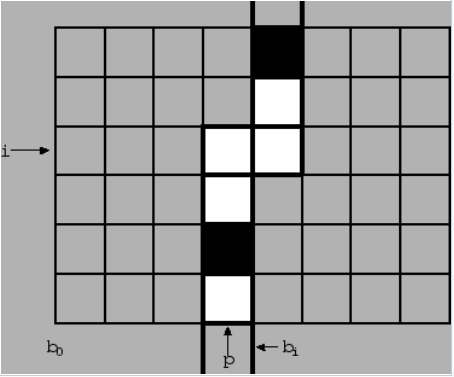
\includegraphics[width=8cm]{images/18-24_alg5.PNG}
\end{center}
Хотим сделать то же самое: предполагая, что все левее разреза покрашено корректно, знать, как будем продолжать красить\\
1. dp[j][i][mask] =  сколько способов дойти до j столбца и  i ячейки в нем, считая сверху, с маской mask у нас есть. (i+1,j) -  излом,  mask - соответственная маска вдоль этого излома (на картинке - раскрашенная полоска)\\
2. База: 
\begin{center}
    
\includegraphics[width=8cm]{images/18-24_alg27.PNG}
\end{center}
, все остальные - 0\\
3. Переход: Просчитываем, как можно изменить квадратик, стоящий на изломе (то есть он может быть 0 или 1). Если преход корректен,красим его в этот цвет, переходим к dp[j][i+1][newmask], где новая маска пересчитывается в соответствии с тем, как мы покрасили клетку. Заметим, что хотябы один переход возможен всегда
\begin{center}
    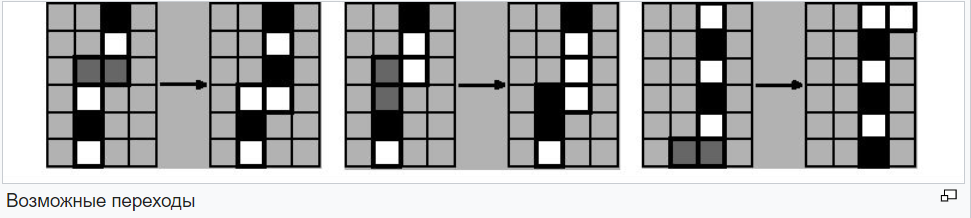
\includegraphics[width=17cm]{images/18-24_alg25.PNG}
\end{center}
Чуть-чуть подробнее про переходы масок. Ячейки в маске нумеруются s-ками. Проталкивая разрез, меняем в маске s+1 ячейку на выбранную раскраску излома, новым изломом становится клеточка под крестиком
\begin{center}
    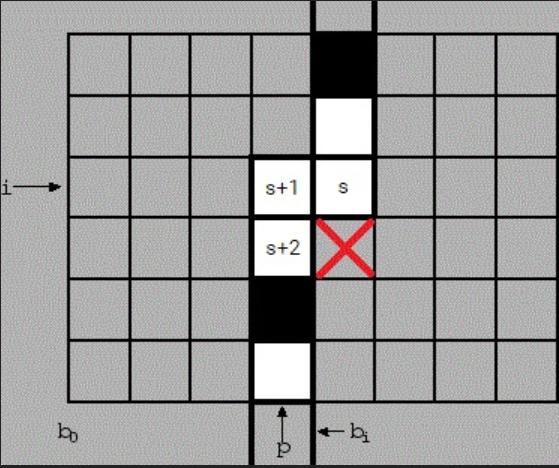
\includegraphics[width=8cm]{images/18-24_alg26.PNG}
\end{center}
Алгоритм:
\begin{itemize}
    \item [1] Цикл по j
    \item [2] Цикл по mask
    \item [3] Цикл по i
    \item [4] Просчитываем квадратик излома
    \begin{itemize}
        \item Если можно поставить единичку или ноль, ставим, получаем newmask, dp[j][i+1][newmask] +=  dp[j][i][mask] (если дошли до конца столбца, переходим в  dp[j+1][1][newmask]
        
    \end{itemize}
\end{itemize}
Ответ: сумма по всем mask dp[m][n][mask]